\documentclass[../../../Bachelorarbeit.tex]{subfiles}
\begin{document}

\subsection{Anforderungsanalyse} \label{anforderungsana}
In der Analysephase der Systementwicklung werden die Kundenanforderungen zusammengetragen und untersucht.
Dabei stellt die Anforderungsanalysephase den ersten Schritt zum Aufstellen der initialen Dokumente für den Prozess dar \cite[333]{Lauber1999}. In weiteren Iterationen liegen der Anforderungsanalyse zusätzlich zu der ursprünglichen Aufgabenstellung noch die Ergebnisse der Tests und die erkannten Analysefehler ebenfalls als Quelle vor.\\
Die ermittelten Anforderungen werden untergliedert in funktionale und nicht-funktionale Anforderungen (kurz \textbf{\acsp{fa}} und \textbf{\acsp{nfa}}) \cite[337]{Lauber1999}. Diese Unterteilung findet in der Arbeit in separaten Unterabschnitten statt, die sich nachfolgend anschließen. Die Identifikation der Stakeholder ist grundsätzlich der Anforderungsanalyse zugehörig, wird jedoch in einem gesonderten, sich der Anforderungsanalyse anschließenden, Unterkapitel behandelt, da es sich im Kontext des Konzeptionsteils dieser Arbeit um einen Kernabschnitt handelt.\\
Zur übersichtlichen Einordnung des jeweiligen Analyseschrittes wird die Grafik Analysephase eingeführt, an der sich die folgenden Kapitel entlangbewegen. Die Anforderungsanalyse kann auf der linken Seite der Grafik identifiziert werden und untergliedert sich in die bereits erwähnten drei Unterpunkte.\\

\begin{figure}[H]
    \centering
    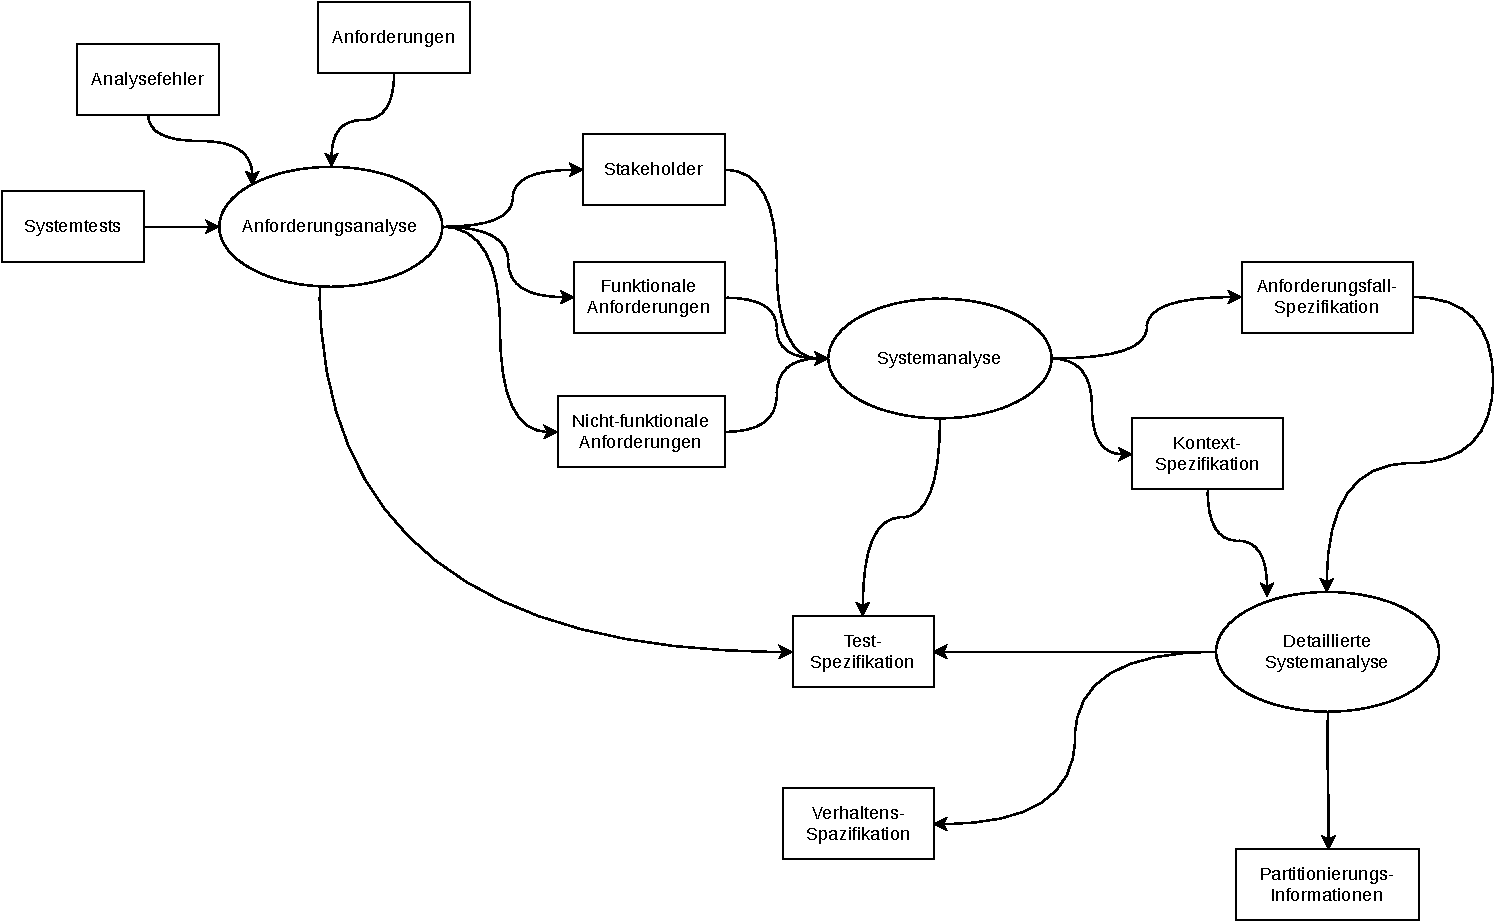
\includegraphics[width=0.9\textwidth]{Images/AnalyseDiagramm.vpd.pdf}
    \caption[Analysephasen]{Diagramm - Analysephasen des Systementwicklungsprozesses \cite[42]{Walke2005}}
    \label{fig:my-img8}
\end{figure}

Die folgenden Abschnitte betrachten die Erstellung einer konkreten Anforderungsspezifikation, die zum Startbeginn des Entwicklungsprozesses vorliegen muss. In den Unterabschnitten zu den \acp{fa} und \acp{nfa} werden die notwendigen Anforderungen für die Entwicklung der Laboranlage vorgestellt. \\
Aus der theoretischen Grundlagen bereits erkenntlich, bestehen Anforderungen aus Zielen, die im Rahmen der Entwicklung erreicht werden sollen. Dabei handelt es sich um einfachen Text, der nach Absprachen mit dem Kunden dokumentiert wird. Konkret geht es im Fall dieser Arbeit um die definierten Aufgaben und Ziele, welche durch Professoren/innen und Laboringenieure/innen \bzw Mitarbeiter/innen des Fachbereiches aufgestellt wurden. Auch selbstauferlegte Aufgaben (Anforderungen des Systementwicklers) werden mit aufgeführt. Im ersten Schritt ist es notwendig die Menge aller Aufgaben zu konkretisieren, um überflüssige und irrelevante Lösungen diese betreffend zu vermeiden.\\
Ausgangspunkt für die Entwicklung des mehrachsigen Positioniersystems sind folgende Kernanforderungen \bzw Ziele. Es wird gefordert, eine Laboranlage zu entwickeln, die simple Transportgüter sicher von einer Aufnahmeposition zu einem Ablageort transportieren kann. Dies soll über zunächst zwei Achsen geschehen, die es ermöglichen Bewegungen in horizontale Richtung (x-Achse) und vertikale Richtung (z-Achse) durchzuführen. Dabei ist es relavant, dass verschiedene Trajektorien von der Anlage gefahren werden können, welche durch den Nutzer programmatisch vorgegeben werden. Die Bewegung der Achsen erfolgt über zwei getrennt ansteuerbare Servomotoren, die über einen Servoregler mit einer Industriesteuerung verbunden sind. Die Steuerungskomponenten sind bereits vorhanden und müssen verwendet werden. Konkret handelt es sich um den \acs{lmc}400c (Logic Motion Controller) von Schneider Electric, das \acs{lxm} 62P Netzgerät (\eng Powersupply, ebenfalls von Schneider Electric) und den \acs{lxm} 62D Doppelantrieb (\eng Double Drive). Zusätzlich soll eine PFC200 Steuerung von Wago zum Einsatz kommen, mit der Betriebsströme gemessen und für die Weiterverarbeitung bereitgestellt werden können. Weiterhin sollen auch ausgewählte Prozessdaten aus dem Systemablauf für die externe Verarbeitung zur Verfügung gestellt werden. Es ist vorgegeben, dass diese Daten per \ac{opc} \ac{ua} Schnittstelle ausgelesen werden können. Kernziel bei der Entwicklung des Laborsystems ist es die Möglichkeit bereitzustellen, dass die Positioniereinheit von jedem Laborplatz programmiert und als Testsystem für den Lehrzweck eingesetzt werden kann. Für den Betrieb der Anlage sind zwei Betriebsmodi vorgesehen. Ersterer, der Automatikbetrieb soll einen vollautomatischen Prozessablauf ermöglichen, bei welchem eine konkrete Positionieraufgabe zyklisch durchgeführt wird. Zweiterer, der Handbetrieb, nimmt manuelle Steuerbefehle vom Nutzer entgegen, bei welchen über Tastereingaben an der Laboranlage, Fahrbewegungen entlang der beiden Achsen durchgeführt werden können. Die Auswahl \bzw ein Wechsel zwischen den Betriebsmodi, ist über einen Wahltaster zu implementieren. Außerdem ist ein Schutz für die Anlage und deren Nutzer, sowie sich um das Positioniersystem befindende Personen zu implementieren. Der Schutz ist manuell auslösbar über Not-Halt Taster an der Laboranlage und durch einen Lichtvorhang vor dem Fahrbereich der beiden Achsen. Abschließend wird gefordert, dass es zu einem späteren Zeitpunkt noch möglich ist, das System um weitere Achsen und Peripheriegeräte wie \bspw Förderbänder zu erweitern.

\subsubsection{Funktionale Anforderungen}
Der erste Unterabschnitt der Anforderungsanalyse behandelt die Modellierung der funktionalen Anforderungen des Prozesses. Im Requirements Engineering beschreiben funktionale Anforderungen gewünschte Funktionalitäten des Systems. Konkret steht im Mittelpunkt der Analyse, welche Fähigkeiten das System besitzen soll \bzw was es umgangssprachlich formuliert tun kann. Die Auflistung der Anforderungen ist eine Sammlung von systemspezifischen Daten, sowie eine grundlegende Beschreibung des Systemverhaltens \cite[338]{Lauber1999}. \\
Die Dokumentation der funktionalen Anforderungen erfolgt typischerweise in Tabellenform. Bereits in den Anforderungen wird ein Abnahmekriterium für diese formuliert, um bei der Inbetriebnahme des Systems die Erfüllung der Anforderung bestätigen oder widerlegen zu können \cite[55]{Kleuker2013}.\\
Die Nachfolgenden Tabellen zu den funktionalen Anforderungen sind wie folgt strukturiert. Der erste Eintrag, die \textbf{Identifikationsnummer} (kurz \acs{id}) dient zum späteren Referenzieren und leichterem Nachschlagen einer Anforderung. Sie ist hilfreich, um Mehrdeutigkeiten zu vermeiden und eine eindeutige Identifizierung sicherzustellen. Im nächsten Punkt, der \textbf{Beschreibung}, wird zunächst in kurzer Textform die Anforderung an das System formuliert. Der Eintrag \textbf{Begründung} enthält Informationen zur Relevanz der Anforderung, die in der Tabelle beschrieben wird. Dem Punkt\textbf{Abhängigkeit} unterliegt eine besondere Wichtigkeit, da hier alle Anforderungen aufgelistet sind, die auf der in der Tabelle beschriebenen Anforderung basieren \bzw in direkter Abhängigkeit zu dieser stehen. Im nächsten Punkt, dem \textbf{Abnahmekriterium} findet eine Erklärung zur Überprüfung der Umsetzung behandelter Anforderung statt. Die Tabellenzeile \textbf{Quelle} verweist auf einen oder mehrere Einträge in der Stakeholdertabelle, welche im \autoref{stakeholder} vorgestellt wird. Bei Nachfragen zu der jeweils behandelten funktionalen Anforderung ist die Tabelle zur Klärung durch den Prozessentwickler heranzuziehen \cite[56]{Kleuker2013}. \\
Die nachfolgenden Tabellen folgen dem beschriebenen Muster und beinhalten alle funktionalen Anforderungen des mehrachsigen Positioniersystems.\\  Die Anforderungen an die Hardware des Systems sind nur beispielhaft am Ende des Unterabschnittes erwähnt. Alle nicht erwähnten Anforderungen können im Anhang nachgeschlagen werden.
Begonnen wird mit funktionalen Anforderungen die Steuerung und Bedienung das System betreffend. Dabei steht im Zentrum der Anforderungsanalyse zunächst die Interaktion des Nutzers mit dem Positioniersystem. Die ersten sieben Anforderungen beschreiben die Hardwareelemente am Schaltschrank und die Reaktionen des Systems nach Betätigung der Bedienelemente.
% FA - Einschalter
\begin{table}[H]
    \centering
    \begin{tabular}{ p{0.34\linewidth}  p{0.6\linewidth} }
        \hline
        \textbf{Identifikationsnummer}  & \multicolumn{1}{r}{FA\_01} \\ \hline
        \textbf{Beschreibung}           & Das Positioniersystem soll über einen dedizierten Einschalter unter Spannung gesetzt werden können. \\
        \textbf{Begründung}             & Es wird verlangt, bei Nichtnutzung des Systems dieses zu deaktivieren um das Gefahrenrisiko zu minimieren. \\
        \textbf{Abhängigkeit}           &   {\begin{itemize}[noitemsep,topsep=0pt,parsep=0pt,partopsep=0pt,leftmargin=*]
                                                \item Auswahl des Betriebsmodus (siehe \autoref{tab:my-table2} \textit{FA\_02}).
                                                \item Es sind Schutzmaßnahmen für Anwender und Anlage umzusetzen, um das Gefahrenrisiko zu minimieren (siehe \autoref{tab:my-table13} \textit{NFA\_07} und \autoref{tab:my-table15} \textit{NFA\_09}).
                                            \end{itemize}} \\
        \textbf{Abnahmekriterium}       & Die Steuerungskomponenten fahren hoch, was über das Aufleuchten der \textit{Power-LED} am \acs{lmc} bestätigt werden kann. Weiterhin leuchtet der rote \textit{STOP-Taster} (Signalisiert den gestoppten Zustand des Systems). \\
        \textbf{Quelle}                 & Laborpersonal siehe Stakeholderliste \\ \hline
    \end{tabular}
    \caption[\acs{fa} - EIN-Schalter]{Funktionale Anforderung - Ein-Schalter}
    \label{tab:my-table}
\end{table}
% FA Wahlschalter Betriebsmodus
\begin{table}[H]
    \centering
    \begin{tabular}{ p{0.34\linewidth}  p{0.6\linewidth} }
        \hline
        \textbf{Identifikationsnummer}  & \multicolumn{1}{r}{FA\_02} \\ \hline
        \textbf{Beschreibung}           & Über einen Wahlschalter soll der Betriebsmodus des mehrachsigen Positioniersystems vorgegeben werden können. \\
        \textbf{Begründung}             & Es ist hilfreich die Auswahl zwischen dem Normalbetrieb (Automatikbetrieb) und einem sogenannten Handbetrieb zu haben, in dem das System einfacher kalibriert und auf seine Funktionalität geprüft werden kann. \\
        \textbf{Abhängigkeit}           & Auswahlbestätigung des Betriebsmodus über \textit{START-Taster} (siehe \autoref{tab:my-table2.5} \textit{FA\_03}) \\
        \textbf{Abnahmekriterium}       & Auswahl des Handmodus wird über das Aufleuchten der weißen Taster am Schaltschrank indiziert. Die Visualisierung zeigt den aktuellen Betriebsmodus als grün hinterlegt. \\
        \textbf{Quelle}                 & Prozessentwickler siehe Stakeholderliste \\ \hline
    \end{tabular}
    \caption[\acs{fa} - Wahlschalter Betriebsmodus]{Funktionale Anforderung - Wahlschalter Betriebsmodus}
    \label{tab:my-table2}
\end{table}
% FA START-Taster
\begin{table}[H]
    \centering
    \begin{tabular}{ p{0.34\linewidth}  p{0.6\linewidth} }
        \hline
        \textbf{Identifikationsnummer}  & \multicolumn{1}{r}{FA\_03} \\ \hline
        \textbf{Beschreibung}           & Über einen grünen \textit{START-Taster} soll der ausgewählte Betriebsmodus bestätigt \bzw ausgeführt werden. Der \textit{START-Taster} dient gleichzeitig auch als \textit{RESET-Taster}, um nach einem Not-Halt-Ereignis das System wieder zu reaktivieren (resetten). \\
        \textbf{Begründung}             & Über die Auswahlbestätigung des Modus kann sichergestellt werden, dass nicht versehentlich der Modus gewechselt wurde (zweistufige Bestätigung). Das Reaktivieren des Positioniersystems nach einem Fehler erfolgt über den gleichen Taster (gleiche Funktionalität). \\
        \textbf{Abhängigkeit}           &   {\begin{itemize}[noitemsep,topsep=0pt,parsep=0pt,partopsep=0pt,leftmargin=*]
                                                \item Resetten des Systems nach Not-Halt (siehe \autoref{tab:my-table2.8} \textit{FA\_06}).
                                                \item Abarbeitung des Automatikmodus (siehe \autoref{tab:my-table2.10} \textit{FA\_08}).
                                                \item Betriebsbereitschaft im Handmodus (Erwarten von Eingabebefehlen siehe \autoref{tab:my-table2.6} \textit{FA\_04} und \autoref{tab:my-table2.7} \textit{FA\_05})
                                            \end{itemize}} \\
        \textbf{Abnahmekriterium}       & \textit{START-Taster} leuchtet grün auf und roter \textit{STOP-Taster} erlischt. Falls die Auswahl des Automatikmodus bestätigt wurde, beginnt die Abarbeitung der einzelnen Schritte des Normalbetriebs. Wurde der Handmodus ausgewählt, können nun über die vier schwarzen Richtungsgeber-Taster oder die zwei weiß leuchtenden Taster am Schaltschrank manuell Anlagenfunktionen aktiviert \bzw ausgeführt werden. \\
        \textbf{Quelle}                 & Studenten siehe Stakeholderliste \\ \hline
    \end{tabular}
    \caption[\acs{fa} - START-Taster]{Funktionale Anforderung - START-Taster}
    \label{tab:my-table2.5}
\end{table}
% FA Richtungsgeber-Taster (Handmodus)
\begin{table}[H]
    \centering
    \begin{tabular}{ p{0.34\linewidth}  p{0.6\linewidth} } 
        \hline
        \textbf{Identifikationsnummer}  & \multicolumn{1}{r}{FA\_04} \\ \hline
        \textbf{Beschreibung}           & Über Tastereingaben an einem Vier-Wege-Richtungsgeber soll es möglich sein die beiden Achsen im Handmodus zu bewegen (joggen). \\
        \textbf{Begründung}             & Der Handmodus erfordert manuelle Nutzereingaben. Dieser erfolgen über die besagten Richtungsgeber-Taster. Alternativ kann die selbe Funktionalität auch über die Visualisierung ausgeführt werden. \\
        \textbf{Abhängigkeit}           &   {\begin{itemize}[noitemsep,topsep=0pt,parsep=0pt,partopsep=0pt,leftmargin=*]
                                                \item Die Bewegung der Achsen erfolgt innerhalb des durch die Endlagesensoren abgesteckten Fahrbereiches (siehe \autoref{tab:my-table5} \textit{FA\_12}).
                                                \item Die Bewegung der Achsen ist verlangsamt in Endlagennähe (geringere Beschleunigung und Geschwindigkeit) (siehe \autoref{tab:my-table6} \textit{FA\_13}).
                                            \end{itemize}} \\
        \textbf{Abnahmekriterium}       & Tasteingaben auf dem Vier-Wege-Richtungsgeber führen im bestätigten Handbetrieb zu Bewegungen der jeweils angesteuerten Achse. \\
        \textbf{Quelle}                 & Lehrpersonal siehe Stakeholderliste \\ \hline
    \end{tabular}
    \caption[\acs{fa} - Bewegungssteuerung im Handmodus]{Funktionale Anforderung - Bewegungssteuerung im Handmodus}
    \label{tab:my-table2.6}
\end{table}
% FA Greifer-Taster (Handmodus)
\begin{table}[H]
    \centering
    \begin{tabular}{ p{0.34\linewidth}  p{0.6\linewidth} } 
        \hline
        \textbf{Identifikationsnummer}  & \multicolumn{1}{r}{FA\_05} \\ \hline
        \textbf{Beschreibung}           & Über die Betätigung von zwei weißen Tastern am Schaltschrank soll zum Einen ein auf der z-Achse befestigter Greifarm umgeschwenkt werden können, zum anderen soll ein Greifer geöffnet und geschlossen werden, um Transportobjekte aufzunehmen/abzulegen. \\
        \textbf{Begründung}             & Der Handmodus erfordert manuelle Nutzereingaben. Dieser erfolgen über besagte zwei weiße Taster zur Steuerung des Greifens. Alternativ kann die selbe Funktionalität auch über die Visualisierung ausgeführt werden. \\
        \textbf{Abhängigkeit}           & Ablage von Transportobjekten auf Ablagepositionen oder Weitergabe von Transportobjekten an \zB ein Förderband (spätere Erweiterung) \\ 
        \textbf{Abnahmekriterium}       & Es können sowohl Objekte links als auch rechts von der Positioniereinheit gegriffen und abgelegt werden. \\
        \textbf{Quelle}                 & Prozessentwickler siehe Stakeholderliste \\ \hline
    \end{tabular}
    \caption[\acs{fa} - Greifen von Transportobjekten im Handmodus]{Funktionale Anforderung - Greifen von Transportobjekten im Handmodus}
    \label{tab:my-table2.7}
\end{table}
% FA Resetten nach Not-Halt
\begin{table}[H]
    \centering
    \begin{tabular}{ p{0.34\linewidth}  p{0.6\linewidth} } 
        \hline
        \textbf{Identifikationsnummer}  & \multicolumn{1}{r}{FA\_06} \\ \hline
        \textbf{Beschreibung}           & Durch Betätigung des \textit{RESET-Tasters} (gleichzeitig auch der grüne \textit{START-Taster}) soll das System nach einem Not-Halt wieder reaktiviert werden, um anschließend normal genutzt werden zu können. \\
        \textbf{Begründung}             & Die Wiederaufnahme der Abarbeitung der Anlagenfunktionen sollte erst nach manueller Bestätigung, dass der Fehler \bzw die Notsituation beseitigt ist, stattfinden. \\
        \textbf{Abhängigkeit}           & Es sind Schutzmaßnahmen für Anwender und Anlage umzusetzen, um das Gefahrenrisiko zu minimieren(siehe \autoref{tab:my-table13} \textit{NFA\_07} und \autoref{tab:my-table15} \textit{NFA\_09}). \\
        \textbf{Abnahmekriterium}       & Es können sowohl Objekte links als auch rechts von der Positioniereinheit gegriffen und abgelegt werden. \\
        \textbf{Quelle}                 & Studenten siehe Stakeholderliste \\ \hline
    \end{tabular}
    \caption[\acs{fa} - RESET-Taster]{Funktionale Anforderung - RESET-Taster}
    \label{tab:my-table2.8}
\end{table}
% FA Geschwindigkeitsregulierung
\begin{table}[H]
    \centering
    \begin{tabular}{ p{0.34\linewidth}  p{0.6\linewidth} } 
        \hline
        \textbf{Identifikationsnummer}  & \multicolumn{1}{r}{FA\_07} \\ \hline
        \textbf{Beschreibung}           & Die Geschwindigkeit der beiden Achsen soll jeweils durch ein Potentiometer am Schaltschrank vorgegeben werden. \\
        \textbf{Begründung}             & Das Regulieren der Fahrgeschwindigkeit erleichtert auf der einen Seite die Identifikation von Fehlern (langsames Fahren), auf der anderen Seite kann die Dauer von Positionieraufgaben verringert werden (schnelleres Fahren). \\
        \textbf{Abhängigkeit}           & --- \\
        \textbf{Abnahmekriterium}       & Das Einstellen von Geschwindigkeiten über die Potentiometer an der Schaltschrankfront führt zur Änderung der Fahrgeschwindigkeit der jeweiligen Achse. \\
        \textbf{Quelle}                 & Prozessentwickler siehe Stakeholderliste \\ \hline
    \end{tabular}
    \caption[\acs{fa} - Regulierung der Fahrgeschwindigkeit]{Funktionale Anforderung - Regulierung der Fahrgeschwindigkeit}
    \label{tab:my-table2.9}
\end{table}

Anschließend an die funktionalen Anforderungen die Systembedienung betreffend, folgt nun die Anforderung zur Funktionalität des Systems im Automatikmodus, welcher den Normalbetrieb des Systems darstellen soll. Bei dieser Anforderung handelt es sich um eine der Kernanforderungen an das System. Erweitert wird diese um die Anforderung, dass der Fahrweg \bzw die Trajektorie der Achsenbewegungen programmatisch vorgegeben werden kann.

% FA Abarbeitung Automatikmodus
\begin{table}[H]
    \centering
    \begin{tabular}{ p{0.34\linewidth}  p{0.6\linewidth} } 
        \hline
        \textbf{Identifikationsnummer}  & \multicolumn{1}{r}{FA\_08} \\ \hline
        \textbf{Beschreibung}           & Nach bestätigter Auswahl des Automatikmodus soll das System vollautomatisch Positionier- und Greifaufgaben durchführen. Es sollten beispielsweise Koordinatenpunkte angefahren werden, um dort Greifaktionen auszuführen. \\
        \textbf{Begründung}             & Im Automatikmodus soll das System selbstständig ohne Erfordernis von Nutzereingaben ein vorgegebenes Programm abarbeiten. \\
        \textbf{Abhängigkeit}           &   {\begin{itemize}[noitemsep,topsep=0pt,parsep=0pt,partopsep=0pt,leftmargin=*]
                                                \item Die Bewegung der Achsen erfolgt innerhalb des durch die Endlagesensoren abgesteckten Fahrbereiches(siehe \autoref{tab:my-table5} \textit{FA\_12}).
                                                \item Die Bewegung der Achsen ist verlangsamt in Endlagennähe (geringere Beschleunigung und Geschwindigkeit) (siehe \autoref{tab:my-table6} \textit{FA\_13}).
                                                \item Kollisionen mit virtuellen Hindernissen sollen verhindert und der Fahrweg somit angepasst werden (siehe \autoref{tab:my-table2.11} \textit{FA\_09}).
                                            \end{itemize}} \\
        \textbf{Abnahmekriterium}       & Die beiden Achsen des Systems können absolut positioniert werden. Die Positionierung der Achsen erfolgt ohne Nutzereingaben. \\
        \textbf{Quelle}                 & Prozessentwickler, Lehrpersonal siehe Stakeholderliste \\ \hline
    \end{tabular}
    \caption[\acs{fa} - Abarbeitung Automatikmodus]{Funktionale Anforderung - Abarbeitung des Automatikmodus}
    \label{tab:my-table2.10}
\end{table}
% FA Fahrverhalten
\begin{table}[H]
    \centering
    \begin{tabular}{ p{0.34\linewidth}  p{0.6\linewidth} } 
        \hline
        \textbf{Identifikationsnummer}  & \multicolumn{1}{r}{FA\_09} \\ \hline
        \textbf{Beschreibung}           & Durch programmatisches Eingreifen soll das Fahrverhalten (\zB Trajektorien) vorgegeben \bzw angepasst werden können. \\
        \textbf{Begründung}             & Durch die Möglichkeit Fahrparameter und somit auch Trajektorien anpassen zu können, wird es möglich verschiedene Bewegungsparameter zu testen und diese miteinander zu vergleichen. Dadurch ergibt sich ein Optimierungspotenzial der Laboranlage. Weiterhin kann somit eine Umsetzung zur Kollisionsvermeidung von virtuellen Hindernissen umgesetzt werden. \\
        \textbf{Abhängigkeit}           & Programmierschnittstelle zu den Laborcomputern (siehe \autoref{tab:my-table11} \textit{NFA\_05}). \\
        \textbf{Abnahmekriterium}       & Der Fahrweg zwischen einem Start- und Endpunkt wurde erfolgreich angepasst und das System führt abweichende Bewegungsmuster aus. \\
        \textbf{Quelle}                 & Lehrpersonal siehe Stakeholderliste \\ \hline
    \end{tabular}
    \caption[\acs{fa} - Anpassung des Fahrverhaltens]{Funktionale Anforderung - Anpassung des Fahrverhaltens}
    \label{tab:my-table2.11}
\end{table}

Die letzten vier funktionalen Anforderungen beinhalten allgemeine Informationen das Systemverhalten betreffend und gelten als grundlegende Voraussetzung für die Funktionalität des Positioniersystems. Es ist dabei nicht relevant, ob die Anlage im Hand- oder Automatikmodus betrieben wird.

% FA Positionieren auf zwei Achsen
\begin{table}[H]
    \centering
    \begin{tabular}{ p{0.34\linewidth}  p{0.6\linewidth} }
        \hline
        \textbf{Identifikationsnummer}  & \multicolumn{1}{r}{FA\_10} \\ \hline
        \textbf{Beschreibung}           & Das Positioniersystem soll zwei bewegbare Achsen besitzen, die sich getrennt steuerbar horizontal und vertikal auf ihrem jeweiligen Profil bewegen können. \\
        \textbf{Begründung}             & Um Positionieraufgaben durchführen zu können, sollen Linearachsen zum Einsatz kommen, auf denen \bzw durch welche Bewegungen durchgeführt werden können. \\
        \textbf{Abhängigkeit}           &   {\begin{itemize}[noitemsep,topsep=0pt,parsep=0pt,partopsep=0pt,leftmargin=*]
                                                \item Bewegung der beiden Achsen im Handmodus (siehe \autoref{tab:my-table2.6} \textit{FA\_04}).
                                                \item Abarbeitung des Automatikmodus (siehe \autoref{tab:my-table2.10} \textit{FA\_08}).
                                                \item Anpassung des Fahrweges \bzw der Trajektorie (siehe \autoref{tab:my-table2.11} \textit{FA\_09}).
                                            \end{itemize}} \\
        \textbf{Abnahmekriterium}       & Das System besitzt zwei Achsen mit jeweils einem Servoantrieb pro Achse (Sichtprüfung). \\
        \textbf{Quelle}                 & Lehrpersonal siehe Stakeholderliste \\ \hline
    \end{tabular}
    \caption[\acs{fa} - Positionieren auf zwei Achsen]{Funktionale Anforderung - Positionieren auf zwei Achsen}
    \label{tab:my-table3}
\end{table}
% FA Bremsen der Achsen
\begin{table}[H]
    \centering
    \begin{tabular}{ p{0.34\linewidth}  p{0.6\linewidth} }
        \hline
        \textbf{Identifikationsnummer}  & \multicolumn{1}{r}{FA\_11} \\ \hline
        \textbf{Beschreibung}           & Bewegungen auf den zwei Linearachsen sollen gebremst werden können. \\
        \textbf{Begründung}             & Bewegungen entlang der Achsen müssen auch wieder gestoppt werden können. Weiterhin sollten keine Bewegungen verursacht durch das Gewicht des Systems selbst oder von Transportobjekten auftreten. \\
        \textbf{Abhängigkeit}           &   {\begin{itemize}[noitemsep,topsep=0pt,parsep=0pt,partopsep=0pt,leftmargin=*]
                                                \item Es sollen Endlagesensoren eingesetzt werden (siehe \autoref{tab:my-table5} \textit{FA\_12}).
                                                \item Es sind Schutzmaßnahmen für Anwender und Anlage umzusetzen, um das Gefahrenrisiko zu minimieren (siehe \autoref{tab:my-table13} \textit{NFA\_07} und \autoref{tab:my-table15} \textit{NFA\_09}).
                                            \end{itemize}} \\
        \textbf{Abnahmekriterium}       & Sowohl ein Erreichen von Endlagepositionen, sowie Start- und Zielpositionen, die Nichtbetätigung von Bewegungstastern im Handmodus und das Auslösen des Not-Halts führen zu einem Bremsvorgang und abschließendem Halten der Achsen. Im gestoppten Zustand befindet sich die Anlage im Stillstand und kann nicht bewegt werden. \\
        \textbf{Quelle}                 & Lehrpersonal siehe Stakeholderliste \\ \hline
    \end{tabular}
    \caption[\acs{fa} - Bremsen der Achsbewegungen]{Funktionale Anforderung - Bremsen der Achsbewegungen}
    \label{tab:my-table4}
\end{table}
% FA Endlagen
\begin{table}[H]
    \centering
    \begin{tabular}{ p{0.34\linewidth}  p{0.6\linewidth} } 
        \hline
        \textbf{Identifikationsnummer}  & \multicolumn{1}{r}{FA\_12} \\ \hline
        \textbf{Beschreibung}           & Es sollen induktive Endlagesensoren (Öffner) verbaut werden, die Bewegungen nach Erreichen der Enden der jeweiligen Achse verhindern. \\
        \textbf{Begründung}             & Damit es nicht zu Beschädigungen der Anlage kommt, muss verhindert werden, dass sich die Schlitten auf den Profilen der Achsen über den maximalen Fahrtweg hinaus bewegen können. \\
        \textbf{Abhängigkeit}           & Es sind Schutzmaßnahmen für Anwender und Anlage umzusetzen, um das Gefahrenrisiko zu minimieren (siehe \autoref{tab:my-table13} \textit{NFA\_07} und \autoref{tab:my-table15} \textit{NFA\_09}). \\
        \textbf{Abnahmekriterium}       & Bei Erreichen einer Endlage bewegt sich der jeweilige Schlitten nicht mehr weiter (über die Endlage hinaus), auch dann nicht, wenn die Eingabe für eine Bewegung in diese Richtung erfolgt. Das Vorhandensein der Sensorik wird per Sichtprüfung bestätigt. \\
        \textbf{Quelle}                 & Lehrpersonal siehe Stakeholderliste \\ \hline
    \end{tabular}
    \caption[\acs{fa} - Nutzung induktiver Endlagesensoren]{Funktionale Anforderung - Nutzung induktiver Endlagesensoren}
    \label{tab:my-table5}
\end{table}
% FA Geschwindigkeit Endlagennähe
\begin{table}[H]
    \centering
    \begin{tabular}{ p{0.34\linewidth}  p{0.6\linewidth} } 
        \hline
        \textbf{Identifikationsnummer}  & \multicolumn{1}{r}{FA\_13} \\ \hline
        \textbf{Beschreibung}           & Sowohl die Geschwindigkeit als auch die Beschleunigung der Achsen sollte in Endlagennähe verringert werden. \\
        \textbf{Begründung}             & Ein zu langer Bremsweg aufgrund einer zu großen Geschwindigkeit könnte in Endlagennähe zur Beschädigung der Anlage führen. \\
        \textbf{Abhängigkeit}           & Es sind Schutzmaßnahmen für Anwender und Anlage umzusetzen, um das Gefahrenrisiko zu minimieren (siehe \autoref{tab:my-table13} \textit{NFA\_07} und \autoref{tab:my-table15} \textit{NFA\_09}). \\
        \textbf{Abnahmekriterium}       & Die Bewegung der beiden Achsen ist in Nähe der Endlagen ersichtlich langsamer. \\
        \textbf{Quelle}                 & Lehrpersonal siehe Stakeholderliste \\ \hline
    \end{tabular}
    \caption[\acs{fa} - Entschleunigung in Endlagenähe]{Funktionale Anforderung - Entschleunigung in Endlagenähe}
    \label{tab:my-table6}
\end{table}

% TODO: erweitern um alle restlichen funktionalen Anforderungen

\subsubsection{Nicht-funktionale Anforderungen}
Dieses Unterkapitel behandelt die Modellierung der nicht-funktionalen Anforderungen in der Anforderungsanalyse. Nicht-funktionale Anforderungen sind Forderungen an die Qualität, in welcher Funktionalitäten zu erbringen sind. Auch Randbedingungen für das System \bzw den Prozess werden mit bei den nicht-funktionalen Anforderungen berücksichtigt \cite[337]{Lauber1999}.\\
Die \textbf{Qualitätsanforderungen} gliedern sich in Zeitanforderungen, Sicherheit für Leib und Leben und Zuverlässigkeit sowie Verfügbarkeit. Bei \textit{Zeitanforderungen} handelt es sich meist um Reaktionszeiten eines Systems. Dabei wird unterschieden zwischen harten und weichen Zeitanforderungen. Der Verstoß gegen harte Zeitanforderungen kann mitunter sehr gravierend sein, wohingegen das Nichteinhalten von weichen Zeitanforderungen meist nur als Störfaktor gesehen werden kann. Zeitanforderungen finden sich im Entwicklungsprozess überwiegend in der Beschreibung von Systemprozessen oder in Aktivitäten des Zustandsdiagrammes wieder.\\
Anforderungen bezüglich \textit{Zuverlässigkeit und Verfügbarkeit} treten in der Modellierung in den Knoten des Verteilungsdiagrammes oder fließen in die Systembeschreibung ein.\\
In die Klasse der Anforderungen bezüglich \textit{Sicherheit für Leib und Leben} fällt die Risikovermeidung von Schäden an Menschen, Produkten und die Umwelt.\\
Abschließend werden die \textbf{Randbedingungen} das System betreffend als Sonderklasse der nicht-funktionalen Anforderungen betrachtet. Man unterteilt diese in zwei Kategorien. Es wird unterschieden zwischen Bedingungen, die sich auf das System und Bedingungen, die sich auf den Entwicklungsprozess auswirken.\\
Erstere sind Technologievorgaben, physikalische Anforderungen, Umweltanforderungen und Vorgaben für die Einbettung und Verteilung des Systems. Sowohl Technologievorgaben als auch Vorgaben an die Einbettung und Verteilung fließen direkt in die Modellierung ein. So werden \bspw Nachbarsysteme im Kontextdiagramm und Forderungen nach bestimmter Hardware im Verteilungsdiagramm aufgeführt. Zu den physikalischen Anforderungen zählen \zB Aussagen über das Gehäuse \bzw die Räumlichkeit, in die das Produkt am ende der Entwicklung passen muss. Unter Umweltanforderungen versteht man \bspw klimatische Bedingungen, unter denen das System arbeiten muss.\\
Randbedingungen für den (Entwicklungs-) Prozess basieren auf Vorschriften und Traditionen. Dabei meinen Traditionen Vorschriften, die sich aus bereits früheren Entwicklungen einer Firma ergeben haben \cite[46]{Walke2005}.\\
Zuletzt soll an dieser Stelle noch eine entscheidende Problematik, die durch die Modellierung nicht-funktionaler Anforderungen auftritt, Erwähnung finden. Es besteht die Möglichkeit, dass nicht-funktionale Anforderungen entgegensätzliche Dinge verlangen. Um diese Problematik zu beseitigen oder zumindest zu minimieren, hat sich in der Praxis die Vergabe von Prioritäten bewährt. So kann in Tabellenform eine Prioritätsreihenfolge erstellt werden. Diese hilft dem Entwickler zu entscheiden, wie er sich beim Auftreten eines Konfliktes verhält \cite[33]{Laplante2014}.\\
Da nun auch die theoretische Grundlage zu den nicht-funktionalen Anforderungen ausreichend beleuchtet ist, folgt die tabellarische Auflistung aller nicht-funktionalen Anforderungen des mehrachsigen Positioniersystems.\\ 
\newline
Zunächst werden die Qualitätsanforderungen an das System aufgelistet. Begonnen wird dabei mit den Zeitanforderungen an das Positioniersystem.

% NFA Reaktionszeit des Lichtvorhangs
\begin{table}[H]
    \centering
    \begin{tabular}{ p{0.34\linewidth}  p{0.6\linewidth} } 
        \hline
        \textbf{Identifikationsnummer}  & \multicolumn{1}{r}{NFA\_01} \\ \hline
        \textbf{Beschreibung}           & Das Durchbrechen des Lichtvorhangs sollte zu einer Bremsauslösung nach spätestens 50\si{ms} führen \\
        \textbf{Begründung}             & Damit eine zum Positioniersystem sprintende Person nicht durch die Bewegungen der Achsen verletzt wird, muss ein Bremsvorgang getriggert durch das Eintreten in den Positionierbereich ausgelöst werden. \\
        \textbf{Abhängigkeit}           & Es sind Schutzmaßnahmen für Anwender und Anlage umzusetzen, um das Gefahrenrisiko zu minimieren (siehe \autoref{tab:my-table13} \textit{NFA\_07} und \autoref{tab:my-table15} \textit{NFA\_09}). \\
        \textbf{Abnahmekriterium}       & Der Bremsvorgang wird nach weniger als 50\si{ms} eingeleitet (Bestätigung durch Aufnahme des Zeitlichen Verlaufes und Überprüfung der Parametrierung der sicheren Eingangsklemmen für den Lichtvorhang). \\
        \textbf{Quelle}                 & Lehrpersonal siehe Stakeholderliste \\ \hline
    \end{tabular}
    \caption[\acs{nfa} - Reaktionszeit des Lichtvorhangs]{Nicht-Funktionale Anforderung - Reaktionszeit des Lichtvorhangs}
    \label{tab:my-table7}
\end{table}
% NFA Abschaltzeit des Servoreglers
\begin{table}[H]
    \centering
    \begin{tabular}{ p{0.34\linewidth}  p{0.6\linewidth} } 
        \hline
        \textbf{Identifikationsnummer}  & \multicolumn{1}{r}{NFA\_02} \\ \hline
        \textbf{Beschreibung}           & Die Auslösung eines Not-Halts sollte nach spätestens 250\si{ms} zum Abschalten des Servoreglers führen. \\
        \textbf{Begründung}             & Die Abschaltung des Servoreglers verhindert das Weiterfahren der Servomotoren und versetzt diese in einen sicheren Haltezustand. \\
        \textbf{Abhängigkeit}           & Es sind Schutzmaßnahmen für Anwender und Anlage umzusetzen, um das Gefahrenrisiko zu minimieren (siehe \autoref{tab:my-table13} \textit{NFA\_07} und \autoref{tab:my-table15} \textit{NFA\_09}). \\
        \textbf{Abnahmekriterium}       & Der Servoreglers ist nach weniger als 250\si{ms} abgeschaltet (Bestätigung durch Aufnahme des zeitlichen Verlaufes und Überprüfung der Programmierung des Sicherheitsprogrammes). \\
        \textbf{Quelle}                 & Lehrpersonal siehe Stakeholderliste \\ \hline
    \end{tabular}
    \caption[\acs{nfa} - Abschaltzeit des Servoreglers]{Nicht-Funktionale Anforderung - Abschaltzeit des Servoreglers}
    \label{tab:my-table8}
\end{table}
% NFA Bremsdauer der Achsbewegungen
\begin{table}[H]
    \centering
    \begin{tabular}{ p{0.34\linewidth}  p{0.6\linewidth} } 
        \hline
        \textbf{Identifikationsnummer}  & \multicolumn{1}{r}{NFA\_03} \\ \hline
        \textbf{Beschreibung}           & Die Auslösung eines Not-Halts oder einer Endlagedetektierung sollte nach spätestens 200\si{ms} zu einem vollständigen Abbremsen jeglicher Bewegungen der jeweiligen Achse(n) führen (Bewegung ist gestoppt). \\
        \textbf{Begründung}             & Ein zu langer Bremsvorgang könnte zu Personen- oder Anlagenschäden führen \\
        \textbf{Abhängigkeit}           & Es sind Schutzmaßnahmen für Anwender und Anlage umzusetzen, um das Gefahrenrisiko zu minimieren (siehe \autoref{tab:my-table13} \textit{NFA\_07} und \autoref{tab:my-table15} \textit{NFA\_09}). \\
        \textbf{Abnahmekriterium}       & Es findet keine Bewegung mehr nach spätestens 200\si{ms} nach Auslösung des Halt-Ereignisses statt. Die Bestätigung erfolgt über die Messung des zurückgelegten Weges nach Ablauf von 200\si{ms}. \\
        \textbf{Quelle}                 & Lehrpersonal siehe Stakeholderliste \\ \hline
    \end{tabular}
    \caption[\acs{nfa} - Bremsdauer der Achsen]{Nicht-Funktionale Anforderung - Bremsdauer der Achsen}
    \label{tab:my-table9}
\end{table}

Anschließend an die Zeitanforderungen folgen nun drei Anforderungen an die Zuverlässigkeit und Verfügbarkeit des Systems. Abseits der ersten nun folgenden Anforderung handelt es sich um zwei Kernanforderungen an das Systems, welche im Zusammenhang mit der Verfügbarkeit der Laboranlage stehen. Diese soll wie bereits im einleitenden Text des Kapitels beschrieben sowohl von jedem Laborplatz aus programmiert werden können, als auch im Labornetzwerk per OPC UA Daten aus dem Prozess bereitstellen.

% NFA Ausfallhäufigkeit
\begin{table}[H]
    \centering
    \begin{tabular}{ p{0.34\linewidth}  p{0.6\linewidth} }
        \hline
        \textbf{Identifikationsnummer}  & \multicolumn{1}{r}{NFA\_04} \\ \hline
        \textbf{Beschreibung}           & Die Laboranlage sollte maximal einen Systemausfall in 10.000 \si{h} haben. \\
        \textbf{Begründung}             & Das mehrachsige Positioniersystem muss zuverlässig laufen, um sowohl für den Lehrzweck als auch für die Gewinnung von Systemdaten zur Weiterverarbeitung eingesetzt werden zu können. \\
        \textbf{Abhängigkeit}           & --- \\
        \textbf{Abnahmekriterium}       & Dauertest bei Bedarf. Treten Ausfälle bereits nach kurzer Zeit auf, gilt die Anforderung als nicht erfüllt. \\
        \textbf{Quelle}                 & Mitarbeiter der Labore siehe Stakeholderliste \\ \hline
    \end{tabular}
    \caption[\acs{nfa} - Ausfallhäufigkeit]{Nicht-Funktionale Anforderung - Ausfallhäufigkeit}
    \label{tab:my-table10}
\end{table}
% NFA Programmierschnittstelle
\begin{table}[H]
    \centering
    \begin{tabular}{ p{0.34\linewidth}  p{0.6\linewidth} }
        \hline
        \textbf{Identifikationsnummer}  & \multicolumn{1}{r}{NFA\_05} \\ \hline
        \textbf{Beschreibung}           & Es soll die Möglichkeit bereitgestellt werden von jedem Laborcomputer eine Verbindung zur Anlage herzustellen, um \zB die Steuerungssoftware anzupassen. \\
        \textbf{Begründung}             & Für den Einsatz der Laboranlage im Lehrbetrieb muss die Anlage im Labornetzwerk gefunden werden können, um von den Studierenden als Anwendungsbeispiel genutzt werden zu können. \\
        \textbf{Abhängigkeit}           & --- \\
        \textbf{Abnahmekriterium}       & Sämtliche \acsp{sps} des Systems (\acs{lmc}, \acs{slc} und PFC200) können in der Programmierumgebung MachineExpert (LogicBuilder) gefunden und mit Programmen bespielt werden. \\
        \textbf{Quelle}                 & Lehrpersonal siehe Stakeholderliste \\ \hline
    \end{tabular}
    \caption[\acs{nfa} - Programmierschnittstelle]{Nicht-Funktionale Anforderung - Programmierschnittstelle}
    \label{tab:my-table11}
\end{table}
% NFA OPC UA Schnittstelle
\begin{table}[H]
    \centering
    \begin{tabular}{ p{0.34\linewidth}  p{0.6\linewidth} }
        \hline
        \textbf{Identifikationsnummer}  & \multicolumn{1}{r}{NFA\_06} \\ \hline
        \textbf{Beschreibung}           & Der \acs{lmc} soll zusätzlich als OPC UA Server fungieren, über welchen Prozessdaten aus einer globalen Variablenliste ausgegeben werden. Dazu gehören Positionsdaten der beiden Achsen, sowie deren aktuelle Geschwindigkeit und Beschleunigung. Es kann der Status der Bremsen ausgelesen werden und der Betriebsstrom der gesamten Anlage. \\
        \textbf{Begründung}             & Die Laboranlage soll über einen \acs{ar} Server betrachtet werden können, um schneller und anschaulicher Informationen über die Anlage zu erhalten. Außerdem wird das Positioniersystem als Anwendungsbeispiel im OpenBASYS Projekt der Hochschule eingesetzt, bei dem die Anlage über Verwaltungsschalen genutzt werden soll. Dazu ist es nötig interne Variablen (Prozessdaten) nach außen über die OPC-UA-Schnittstelle zugänglich zu machen. \\
        \textbf{Abhängigkeit}           & --- \\
        \textbf{Abnahmekriterium}       & Über einen OPC UA Client kann eine Verbindung zum als OPC UA Server fungierenden \acs{lmc} hergestellt werden. Nach Aufbau der Verbindung ist es dann möglich Prozessdaten zu empfangen und auszulesen \bzw weiterzuverarbeiten. \\
        \textbf{Quelle}                 & Mitarbeiter der Labore siehe Stakeholderliste \\ \hline
    \end{tabular}
    \caption[\acs{nfa} - OPC UA Schnittstelle]{Nicht-Funktionale Anforderung - OPC UA Schnittstelle}
    \label{tab:my-table12}
\end{table}

Es folgen nun nicht-funktionale Anforderungen die Sicherheit von Leib und Leben betreffend. Dies schließt Anforderungen zur Vermeidung von Schäden an der Anlage mit ein. 

% NFA Sicherheit für Leib und Leben
\begin{table}[H]
    \centering
    \begin{tabular}{ p{0.34\linewidth}  p{0.6\linewidth} }
        \hline
        \textbf{Identifikationsnummer}  & \multicolumn{1}{r}{NFA\_07} \\ \hline
        \textbf{Beschreibung}           & Die Gefahr, dass ein Anwender oder eine sich in Anlagennähe befindende Person durch die Bewegung der Positioniereinheit verletzt wird, soll bestmöglich minimiert werden. Dazu sind Not-Halt Taster vorgesehen, die durch den Anwender betätigt werden können. Zusätzlich ist ein Lichtvorhang verbaut, der die Anlage stoppen soll, falls eine Person oder ein Objekt durch diesen in den Gefahrenbereich eindringt. \\
        \textbf{Begründung}             & Die Sicherheit für den Anwender und sich in der Nähe der Anlage befindende Personen hat höchste Priorität. Personenschäden müssen unbedingt verhindert werden. \\
        \textbf{Abhängigkeit}           &   {\begin{itemize}[noitemsep,topsep=0pt,parsep=0pt,partopsep=0pt,leftmargin=*]
                                                \item Signalisierung einer Gefahrensituation (siehe \autoref{tab:my-table14} \textit{NFA\_08}).
                                                \item Verhinderung von Anlagenschäden (siehe \autoref{tab:my-table15} \textit{NFA\_09}).
                                                \item Gehäuseaufbau zum Schutz vor Verletzungen (siehe \autoref{tab:my-table16} \textit{NFA\_10}).
                                            \end{itemize}} \\
        \textbf{Abnahmekriterium}       & Durch die Simulation einer Notsituation in Form der Betätigung eines einrastenden Not-Halt-Tasters oder nach Durchbrechung des Lichtvorhangs muss die Laboranlage unverzüglich Bremsen und in einen haltenden Zustand übergehen. \\
        \textbf{Quelle}                 & Lehrpersonal siehe Stakeholderliste \\ \hline
    \end{tabular}
    \caption[\acs{nfa} - Sicherheit für Leib und Leben]{Nicht-Funktionale Anforderung - Sicherheit für Leib und Leben}
    \label{tab:my-table13}
\end{table}
% NFA Signalisierung Gefahrensituation
\begin{table}[H]
    \centering
    \begin{tabular}{ p{0.34\linewidth}  p{0.6\linewidth} }
        \hline
        \textbf{Identifikationsnummer}  & \multicolumn{1}{r}{NFA\_08} \\ \hline
        \textbf{Beschreibung}           & Es soll eine Signalampel verbaut werden, die eine erhöte Risikosituation signalisiert, wenn das Positioniersystem in Bewegung ist. Die Signalisierung erfolgt durch abwechselndes Blinken der roten und grünen Leuchtelemente. \\
        \textbf{Begründung}             & Einer sich in Anlagennähe befindenden Person ersichtliche Signalisierung einer Gefahrensituation minimiert das Risiko der Verletzung durch die Anlage. \\
        \textbf{Abhängigkeit}           & --- \\
        \textbf{Abnahmekriterium}       & Die Signalampel leuchtet entsprechend des aktuellen Systemzustandes. \\
        \textbf{Quelle}                 & Prozessentwickler siehe Stakeholderliste \\ \hline
    \end{tabular}
    \caption[\acs{nfa} - Signalisierung Gefahrensituation]{Nicht-Funktionale Anforderung - Signalisierung von Gefahrensituationen}
    \label{tab:my-table14}
\end{table}
% NFA Verhinderung von Anlagenschäden
\begin{table}[H]
    \centering
    \begin{tabular}{ p{0.34\linewidth}  p{0.6\linewidth} }
        \hline
        \textbf{Identifikationsnummer}  & \multicolumn{1}{r}{NFA\_09} \\ \hline
        \textbf{Beschreibung}           & Die Beschädigung der Laboranlage durch die Bewegung der Achsen soll bestmöglich verhindert werden. \\
        \textbf{Begründung}             & Die Beschädigung der Positioniereinheit würde sowohl zu Kosten als auch potenziellen Personenschäden führen, was dringlichst vermieden werden muss. \\
        \textbf{Abhängigkeit}           & Kabel zu beweglichen Komponenten müssen in E-Ketten untergebracht werden (siehe \autoref{tab:my-table17} \textit{NFA\_11}). \\
        \textbf{Abnahmekriterium}       & Es wurden alle geforderten Betriebsmittel zu Verhinderung von Schäden durch bewegliche Systemkomponenten verbaut (Endlagesensorik, Puffer zur Minimierung von Auffahrschäden). Weiterhin existiert eine Not-Halt-Funktionalität. \\
        \textbf{Quelle}                 & Mitarbeiter der Labore siehe Stakeholderliste \\ \hline
    \end{tabular}
    \caption[\acs{nfa} - Verhinderung von Schäden an der Anlage]{Nicht-Funktionale Anforderung - Verhinderung von Schäden an der Anlage}
    \label{tab:my-table15}
\end{table}

Abschließend werden die Randbedingungen als nicht-funktionale Anforderungen zusammengetragen. Dabei handelt es sich zum einen um Anforderungen an das Gehäuse, die bis jetzt noch nicht unter den Anforderungen für die Sicherheit von Leib- und Leben aufgeführt wurden. Zum anderen werden Hardware- und Softwarevorgaben an dieser Stelle mit aufgeführt.

% NFA Gehäuseaufbau
\begin{table}[H]
    \centering
    \begin{tabular}{ p{0.34\linewidth}  p{0.6\linewidth} }
        \hline
        \textbf{Identifikationsnummer}  & \multicolumn{1}{r}{NFA\_10} \\ \hline
        \textbf{Beschreibung}           & Die rechte und linke Seite der Laboranlage sollen mit Plexiglasscheiben bestückt werden. Die elektrische Verteilung ist in einem Schaltschrank unterzubringen. \\
        \textbf{Begründung}             & Weder der Anlagenbereich, in dem Positionieraufgaben durchgeführt werden, noch der Anlagenbereich, in dem das Risiko zur Verletzung durch einen elektrischen Schock bestehen dürfen frei zugänglich sein, um Verletzungen zu vermeiden. \\
        \textbf{Abhängigkeit}           & --- \\
        \textbf{Abnahmekriterium}       & Das Positioniersystem ist von den Seiten mit Plexiglas abgeschirmt und die elektrischen Betriebsmittel \bzw deren Anschlüsse sind in einem Schaltschrank untergebracht (Sichtprüfung). \\
        \textbf{Quelle}                 & Mitarbeiter der Labore siehe Stakeholderliste \\ \hline
    \end{tabular}
    \caption[\acs{nfa} - Gehäuseaufbau]{Nicht-Funktionale Anforderung - Gehäuse}
    \label{tab:my-table16}
\end{table}
% NFA E-Ketten
\begin{table}[H]
    \centering
    \begin{tabular}{ p{0.34\linewidth}  p{0.6\linewidth} }
        \hline
        \textbf{Identifikationsnummer}  & \multicolumn{1}{r}{NFA\_11} \\ \hline
        \textbf{Beschreibung}           & Kabel an den beweglichen Bauteilen der Positioniereinheit müssen sicher mitgeführt werden. \\
        \textbf{Begründung}             & Sämtliche Kabel zu beweglichen Systemkomponenten müssen beweglich gelagert werden, da diese sonst mit umliegenden Betriebsmitteln interferieren könnten. Weiterhin wird dadurch verhindert, dass Kabel reißen. \\
        \textbf{Abhängigkeit}           & --- \\
        \textbf{Abnahmekriterium}       & Die Laboranlage besitzt für jede bewegliche Achse eine E-Kette in welchen sich die Kabel der Betriebsmittel der jeweiligen Achse befinden (Sichtprüfung). \\
        \textbf{Quelle}                 & Mitarbeiter der Labore siehe Stakeholderliste \\ \hline
    \end{tabular}
    \caption[\acs{nfa} - Kabelmitführung]{Nicht-Funktionale Anforderung - Kabelmitführung}
    \label{tab:my-table17}
\end{table}
% NFA Betriebsstrommessung
\begin{table}[H]
    \centering
    \begin{tabular}{ p{0.34\linewidth}  p{0.6\linewidth} }
        \hline
        \textbf{Identifikationsnummer}  & \multicolumn{1}{r}{NFA\_12} \\ \hline
        \textbf{Beschreibung}           & Es soll eine zweite \acs{sps} verbaut werden, die über eine Energieklemme verfügt, über welche der Betriebsstrom des Systems gemessen werden kann. \\
        \textbf{Begründung}             & Über die Bereitstellung des aktuellen Stromverbrauches der Anlage können Rückschlüsse über die Effektivität der Anlage geschlossen werden. Da der Verbrauch des Positioniersystems somit bekannt ist, besteht die Möglichkeit Optimierungen an der Laboranlage durchzuführen. Es könnten beispielsweise Trajektorien verbessert werden, sodass weniger Strom benötigt wird für die Bewegungen. \\
        \textbf{Abhängigkeit}           & Der Betriebsstrom \bzw die Leistung, die das System verbraucht soll per OPC UA Client ausgelesen werden (siehe \autoref{tab:my-table12} \textit{NFA\_06}). \\
        \textbf{Abnahmekriterium}       & Über einen OPC-UA-Client kann auch der Betriebsstrom ausgelesen werden. \\
        \textbf{Quelle}                 & Mitarbeiter der Labore siehe Stakeholderliste \\ \hline
    \end{tabular}
    \caption[\acs{nfa} - Betriebsstrommessung]{Nicht-Funktionale Anforderung - Betriebsstrommessung}
    \label{tab:my-table18}
\end{table}
% NFA Räumliche Vorgabe
\begin{table}[H]
    \centering
    \begin{tabular}{ p{0.34\linewidth}  p{0.6\linewidth} }
        \hline
        \textbf{Identifikationsnummer}  & \multicolumn{1}{r}{NFA\_13} \\ \hline
        \textbf{Beschreibung}           & Das mehrachsige Positioniersystem soll im Laborraum G 422 der HTW Berlin an der Rückwand des Raumes aufgebaut und in Betrieb genommen werden. \\
        \textbf{Begründung}             & Da das System dem Fachbereich 1 und dem Themengebiet Automatisierungstechnik und industrielle Kommunikation zugeordnet werden kann, bietet es sich an dieses in einem der entsprechenden Laborräume aufzubauen. Aus platztechnischen Gründen und dem Vorhandensein von kompatibler Hardware (zur Simulation des Systems) ist es erforderlich dieses im Raum G 422 zu installieren. \\
        \textbf{Abhängigkeit}           & --- \\
        \textbf{Abnahmekriterium}       & System ist sichtbar an der Rückwand des Raumes eingebaut (Sichtprüfung). \\
        \textbf{Quelle}                 & Lehrpersonal siehe Stakeholderliste \\ \hline
    \end{tabular}
    \caption[\acs{nfa} - räumliche Vorgabe]{Nicht-Funktionale Anforderung - räumliche Vorgabe}
    \label{tab:my-table19}
\end{table}
% NFA Hardware- und Softwarevorgabe
\begin{table}[H]
    \centering
    \begin{tabular}{ p{0.34\linewidth}  p{0.6\linewidth} }
        \hline
        \textbf{Identifikationsnummer}  & \multicolumn{1}{r}{NFA\_14} \\ \hline
        \textbf{Beschreibung}           & Die Steuerungskomponenten der Laboranlage sind bereits vorhanden und müssen verbaut werden. Die Hauptsteuerung ist der \acs{lmc}400c von Schneider Electric. Zusammen mit dem \acs{lxm} 62P und \acs{lxm} 62D Modul gehört dieser zur PacDrive 3 Produktserie. Sowohl das erwähnte Netzteil (\acs{lxm} 62P) als auch der Servoregler (\acs{lxm} 62D) sollen verbaut werden. Aus den Technologievorgaben ergibt sich die Festlegung der Entwicklungsumgebung zur Programmierung des Systems. Die Inbetriebnahme der Anlagensoftware erfolgt über die Software MachineExpert. Die beiden Servomotoren des mehrachsigen Positioniersystems stammen ebenfalls von Schneider Electric. Es handelt sich um SH3 multiturn Servos mit Bremse. Auch die \acs{sps} für die Strommessung per Energieklemme ist vorgegeben. Es soll eine Wago \acs{sps} der PFC200-Serie verbaut werden. Zur Erweiterung der Ein- und Ausgänge des Systems sind Modicon TM5 Module bereitgestellt worden, die sowohl aus digitalen als auch analogen Baugruppen bestehen. Für die Umsetzung der Sicherheitsfunktionen wird der \acs{slc} von Schneider Electric mit einem sicheren Eingangsmodul und einem sicheren Ausgangsmodul verwendet. Alle Steuerungskomponenten sollen per SERCOS III Bus miteinander kommunizieren. \\
        \textbf{Begründung}             & Die Hardware wurde von besagten Industrieunternehmen gestellt und musste nicht käuflich erworben werden. Da diese somit vorhanden ist und für vergleichbare Systemaufbauten entwickelt wurde, kommt diese im Positioniersystem zur Anwendung. \\
        \textbf{Abhängigkeit}           & --- \\
        \textbf{Abnahmekriterium}       & Vorgegebene Hardware wurde verbaut (Sichtprüfung). \\
        \textbf{Quelle}                 & Lehrpersonal siehe Stakeholderliste \\ \hline
    \end{tabular}
    \caption[\acs{nfa} - Hardwarevorgaben]{Nicht-Funktionale Anforderung - Hardwarevorgaben}
    \label{tab:my-table20}
\end{table}

% TODO: erweitern um alle restlichen nicht-funktionalen Anforderungen!

\end{document}